
%%% Local Variables: 
%%% mode: latex
%%% TeX-master: t
%%% End: 

\chapter{问卷、平台和工具}

本系统设计基于波士顿大学提供的《神经心理学测试长问卷》及其使用说明文档,通过安卓平台进行了设计,硬件设备选择了联想的YOGA Pro2平板,通过实验选择使用了百度语音开放平台的API接口实行语音识别功能,并选择使用阿里云的开放存储服务OSS作为数据存储位置。本章节就这些资料、平台和工具做简要的介绍,并讨论选择使用的原因。

\section{《神经心理学测试长问卷》介绍}

《神经心理学测试长问卷》已经运用超过了十年\footnote{引自“10 Years of the Neuropsychological Test Battery”}。经过数年来的实验和资料的累积,这份问卷也不断更新,除了传统的一些关于记忆力、习题、语言等测试,也加入了绘画、计算等题目。由于其题目的特殊性(需要有人引导和控制,并对病人进行观察),所以一直沿用传统的“纸笔测试”。通过对该测试各项进行综合打分,可以对病人是否患有认知功能障碍进行精准的判断。然而,由于包括的题目类型和数量繁多、结构比较复杂、操作难以学习,虽然该问卷也有建议版本,但整个问卷的完成依旧需要至少4个小时,而实施的医生也至少经过一年的学习和观察才可以真正上岗对病人进行测试。

\begin{table}[htbp]
\centering
\caption{问卷的题目类型说明表(部分)}
\label{tab:ParametersForPandR}
\begin{tabular}[c]{lcccc}
\toprule[1.5pt]
{\heiti 测试类型} & {\heiti 领域} & {\heiti 第一次测试类型} & {\heiti 第二次测试类型}\\\midrule[1pt]
视觉配对 & 记忆力 & 立即复述 & 延时复述\\
语言配对 & 记忆力 & 立即复述 & 延时复述\\
语言学习测试 & 记忆力 & 立即复述 & 延时复述\\
控制口语测试 & 执行力 & 可认可单词数 & -\\
流利分类测试 & 执行力 & 可认可单词数 & -\\
数字串重复测试 & 执行力 & 正确复述的数字串长度 & -\\
\bottomrule[1.5pt]
\end{tabular}
\end{table}

虽然整个问卷系统需要电子信息化,但为了和十多年的实验和研究资料进行匹配和兼容,对设计到平板电脑上的系统需要几乎完全还原纸板系统上的体验,才能保证在这样系统辅助的测试环境与传统纸笔测试的环境相同,才能够保证测试结果和之前统计的结果相对应。

\section{Android平台介绍}

\subsection{Android介绍}

Android(安卓)是基于Linux内核的一款给移动设备设计的操作系统,目前由Google公司进行开发。为了能够通过屏幕直接操作,Android的设计主要是为了触摸屏移动设备(如智能手机或平板电脑),也可以用于一些特定的电视、车辆或穿戴设备(手表等)。用户可以在触摸屏上进行多种触摸操作,如点击,拖动,滑动等等,它也为用户提供虚拟键盘用于一些文字的输入。\footnote{本段部分内容翻译自Android的维基百科主页http://en.wikipedia.org/wiki/Android\_(operating\_system)}。

Android是开源的系统,便于、也吸引了很多开发者在系统上进行更新或开发。目前Android系统已经开发特别成熟,除了精美的界面,还提供非常多的服务,例如WIFI、拍照、录音、文件存储、蓝牙、GPS定位等等,这些服务都可以便于我们对脑健康系统的开发。另外对比IOS系统,Android上开发应用完全免费,且拥有多个便捷的开发工具。Google为Android开发提供了详尽的软件开发工具(称作SDK),包括了调试器、软件库、一系列模拟器,也包含了一些样例代码和入门文档。其提供的软件库包含了很多调用Android服务的接口,例如界面组件、媒体播放器、文件存储读取等等,故在安卓平台上开发一个系统(一个应用APP)是相对容易、便捷的。

\begin{figure}[h]
  \centering
  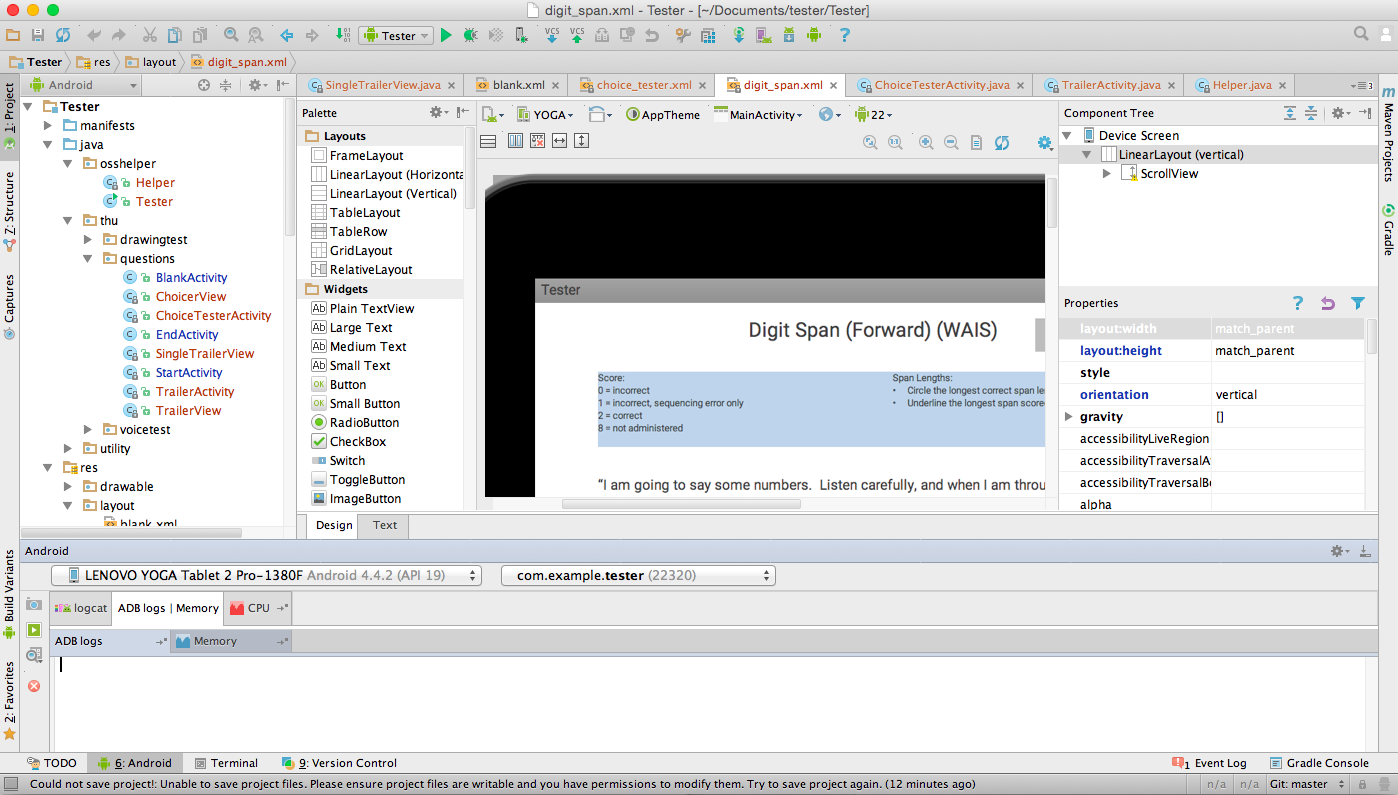
\includegraphics[width=13cm]{chapter1-1}
  \caption{AndroidStudio使用界面}
\end{figure}

\subsection{Android Studio平台介绍}

本次开发Android应用选用了Android Studio这个IDE,它由Google于2013年5月发布,该IDE针对安卓开发,融合了SDK和ADT的版本检查和安装,方便地控制编译的版本;拥有便捷的可视化布局,可以实时编码、实时程序界面浏览;拥有可以协助翻译、优化提示、来源跟踪的开发者控制台,让开发者更舒适地进行编码;基于Gradle地构建支持,也可以方便地和Eclipse开发的Android工程进行相互转化;拥有Android特定的代码重构和快速修复;拥有能对程序性能、可用性、版本兼容等各种问题进行控制捕捉的提示工具;支持应用签名;自带方便的布局编辑器,可以让开发者拖动UI组件,也可以预览在不同设备(可自定义)上UI的显示效果。总体来说,AndroidStudio是一款比Eclipse更便捷、更全面,而又更轻量的的Android开发平台。

\section{联想YOGA平板介绍}

本次系统设计选用的平板电脑为YOGA Pro-1380F,除了拥有其他平板电脑的特点,它拥有13.3英寸的大屏和2560*1440分辨率。基于Android4.4系统深度优化,可以运行所开发的系统。

为了满足“和纸笔测试保持一致”的要求,应用平台应该满足可以记录绘画内容、屏幕大小和标准A4纸相差不打的要求,YOGA Pro-1380F均满足了这些需求。

\begin{figure}[h]
  \centering
  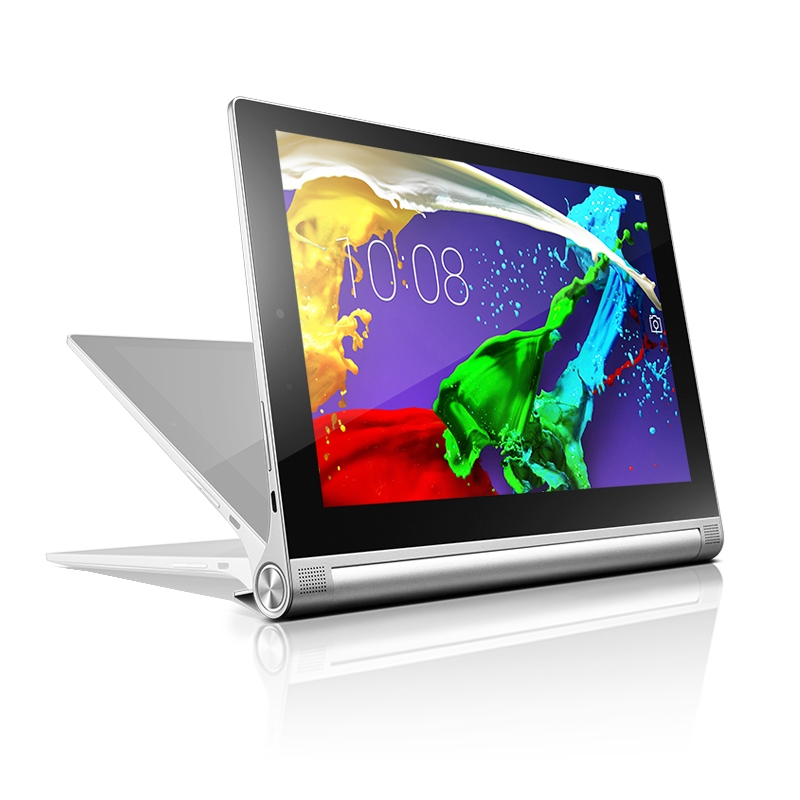
\includegraphics[width=13cm]{chapter1-2}
  \caption{YOGA Pro-1380F}
\end{figure}

\section{阿里云开放存储服务介绍}

阿里云开放存储服务(Open Storage Service,简称OSS)是阿里云对外提供的云存储服务,具有海量、安全、可靠性高的特点。其稳定,系统规模能够在不影响对外服务的前提下自动扩展,数据会进行三重备份,并可以设置日志记录,可靠、丢失易找回;系统通过多层次安全防护,也设置了防DDoS攻击,设有多用户隔离机制,也可以通过日志记录来追查非法访问;为背景用户提供了免费的5GB存储空间,还可以无限量扩展,请求处理能力会根据压力弹性增加,设置了多线BGP网络确保全国各地甚至国外都能访问流畅。另外,阿里云开放存储服务还提供了图片处理的工具,能够对存储在OSS上的图片进行缩略、压缩、裁减、水印和格式转换等图片处理功能。平台提供了详尽了开发者资源(兼容Python,Java,.NET,PHP,iOS,Android,NodeJs)、操作手册和第三方工具,使得基于此平台的开发和数据管理都相当方便。另外官方提供了100倍故障赔偿和全天24小时的售后支持,诸多有名的互联网产品都在此平台上搭建了自己的数据库,如微盟、筋斗云呼叫系统、得图云等等。

本系统的设计所需要的数据类型主要是文字(一些选择选项或是答案)和流媒体(图片,音频或视频),每次测试所生成的数据不超过5MB,故OSS平台提供的5GB的免费空间完全足够开发这个系统测试所需。另外OSS平台的日志记录等特点也适合在开发过程中进行调试;平台提供的Android SDK也为开发提供了便捷的接口,也无需担心服务器地址的移动,同时也利用平台安全、可靠的特性保证了数据的隐密性。故OSS平台是相当适合做该系统数据存储的平台的。

\section{百度语音开放平台介绍}

百度语音开放平台提供了免费的完全永久免费的语音识别服务,不仅支持多种语言(中文、英语、粤语),还提供了基于35个领域的语义解析,依托了百度多个服务(知道、贴吧等社区产品)上累积的强大知识库,能够做到智能推理,提高识别性能。使用场景包括语音搜索、语音输入、语音转写、语音助手等。

本系统的设计在一些语音题上需要运用语音识别系统进行识别,目的在于减少用户对相关文字的输入。通过一系列对目前市场上开放的语音识别服务的评测和实验(后续章节会详细说明),最终选择了百度语音开放平台。


